\documentclass[12pt]{article}
\usepackage{amsmath,setspace,graphicx,amssymb,amsthm,float,esint,tikz}
\usepackage{hyperref}
\usepackage{calligra}

\hypersetup{
    colorlinks,
    allcolors=black
}
\title{\textbf{MATH2106 Electromagnetism Lecture Notes}}
\author{Thomas Piercy}
\date{\today{}}

\newcommand{\df}[2]{\frac{\text{d}#1}{\text{d}#2}}
\newcommand{\seq}[2]{(#1_#2)_{#2\in\mathbb{N}}}
\newcommand{\pf}[2]{\frac{\partial #1}{\partial #2}}
\newcommand{\dive}[1]{\underline{\nabla}\cdot\underline{#1}}
\newcommand{\grad}[1]{\underline{\nabla}#1}
\newcommand{\curl}[1]{\underline{\nabla}\times \underline{#1}}


\DeclareMathAlphabet{\mathcalligra}{T1}{calligra}{m}{n}
\DeclareFontShape{T1}{calligra}{m}{n}{<->s*[2.2]callig15}{}

\newcommand{\scriptr}{\ensuremath{\mathcalligra{r}}\,}
\newcommand{\boldscriptr}{\ensuremath{\pmb{\mathcalligra{r}}}\,}



\begin{document}
\maketitle
\hrulefill
\tableofcontents
\newpage
\setstretch{1.5}
\section{Electrostatics}
\subsection{A Word on Notation}
Most of electromagnetism takes place in \(\mathbb{R}^3\), although unless we are taking a vector product, there is no reason for it to not apply in higher dimensions. Vectors should always be underlined and in a piece of standard physics notation, the same character used but not underlined represents the magnitude of that vector:
\[r=|\underline{r}|\]
Unit vectors are denoted with a hat:
\[\underline{r}=r\,\underline{\hat{r}}\]
Most of electromagnetism will take place in Cartesian coordinates. The Cartesian unit vectors are:
\[\underline{\hat{x}},\ \underline{\hat{y}},\ \underline{\hat{z}}\]
\subsection{Charges}
The SI unit of charge is Coulombs (C). These are defined such that the charge of the electron is:
\[q_e=-e=-1.60\dots\times 10^{-19}\,\text{C}\]
You will not be asked to remember this. In these lectures, a small \(q\) will be used for charges that generate electric fields and a capital \(Q\) will be used for a "test charge" that has forces acting upon it from existing in a field. We are generally interested in the force caused by \(q\) and acting on \(Q\). This force is given to us via Coulombs law:
\[\underline{F}=\frac{1}{4\pi\varepsilon_0}\frac{qQ}{\scriptr^2}\hat{\underline{\scriptr}}=\frac{1}{4\pi\varepsilon_0}\frac{qQ}{|\underline{r}-\underline{r}'|^3}(\underline{r}-\underline{r}')\]
\begin{figure}[H]
    \centering
    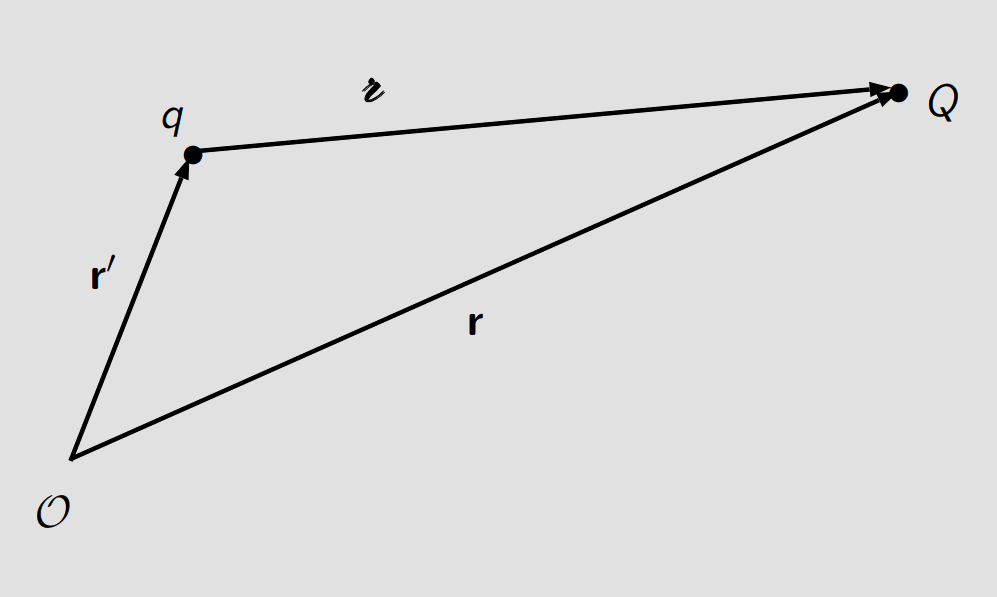
\includegraphics[width=1\linewidth]{Year 2/Images/singlechargeforce.png}
    \caption{A test charge \(Q\) is acted on by a field generated from \(q\).}
\end{figure}
\subsubsection{Observations of Coulombs law}
\begin{itemize}
    \item The magnitude of the force decreases quadratically with the distance between the two charges.
    \item Force is proportional to the product of the charges.
    \item If \(q\) and \(Q\) have the same sign, then the force points away from the field. This is repulsion.
    \item If \(q\) and \(Q\) have opposite signs, then the force points towards the field. This is attraction.
    \item \(\varepsilon_0\) is the vacuum permittivity and is approximately:
    \[\varepsilon_0\approx 8.854\times 10^{-12}\,\frac{\text{C}^2}{\text{Nm}^2} \]
    You do not need to memorise this.
\end{itemize}
\subsubsection{Multiple Charges}
If the force acting on \(Q\) is generated by \(n\) charges \(q_i\), then it is equal to the sum of the forces by the individual charges:
\[\underline{F}=\frac{1}{4\pi\varepsilon_0}\sum^n_{i=1}\frac{q_iQ}{|\underline{r}-\underline{r}_i'|^3}(\underline{r}-\underline{r}_i')\]
\begin{figure}[H]
    \centering
    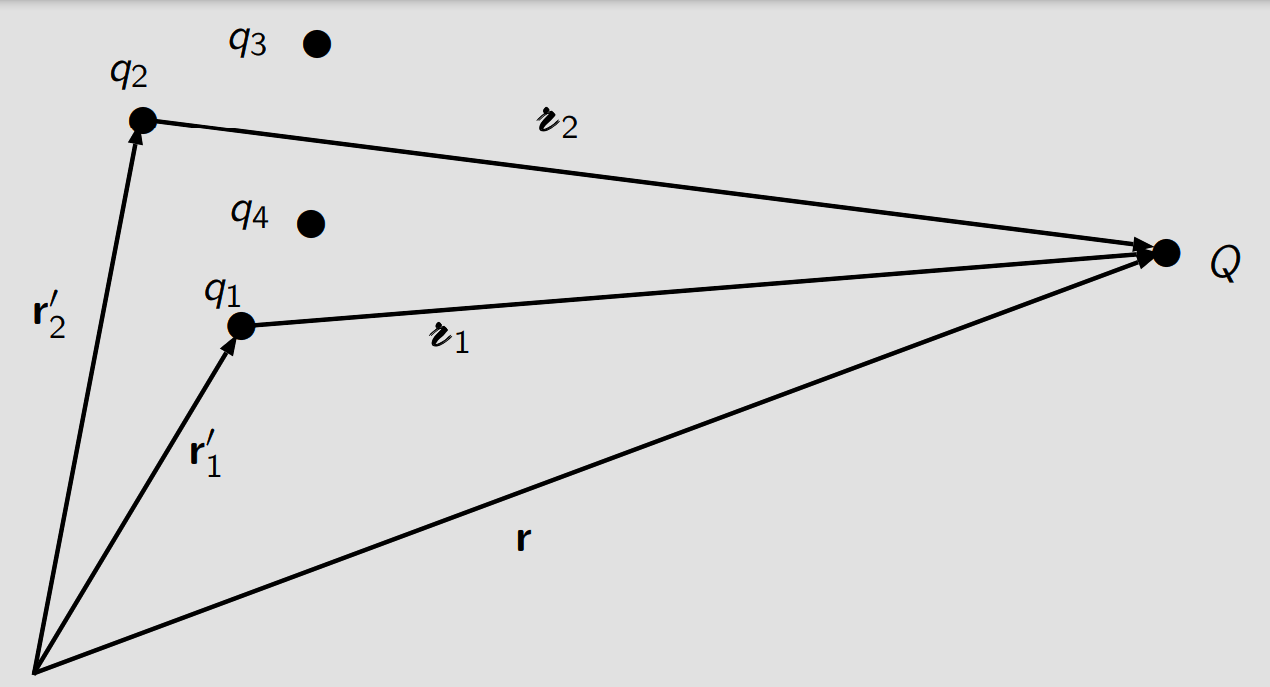
\includegraphics[width=0.75\linewidth]{Year 2/Images/multiplechargeforce.png}
    \caption{A test charge \(Q\), acted on by force generated from multiple charges \(q_i\).}
\end{figure}
Notice that we can take \(Q\) out of the sum and write:
\[\underline{F}=Q\underline{E}\]
Where \(\underline{E}(\underline{r})\) is called the electric field and is defined as:
\[\underline{E}(\underline{r})=\frac{1}{4\pi\varepsilon_0}\sum^n_{i=1}\frac{q_i}{\scriptr^2}\hat{\underline{\scriptr}}\]
\subsection{Continuous Charge Distributions}
Coulombs law doesn't restrict us to just working with discrete sums (although in reality electrons are point charges). In particular if we have a field with lots of charges we may need to look at continuous charge distributions:
\[\underline{E}(\underline{r})=\int\frac{1}{4\pi\varepsilon_0}\frac{1}{\scriptr^2}\hat{\underline{\scriptr}}\,\text{d}q\]
The actual form of this integral will depend on where the charges are located. For example we could have a line or surface integral. If the charge is concentrated on a curve, then define the charge density \(\lambda\):
\[\text{d}q=\lambda \text{d}\ell\]
In this case \(\ell\) is some length parameter along the curve.
\subsubsection{Line charges}
We can construct the electric field for a continuous charge distributions where our charges form a line. Notice that the force acting on a test charge from this line decreases with distance and indeed if the distance from the line is significantly larger than the line itself then it just appears like a point charge at the origin.
\subsubsection{Spherical coordinate recap}
Recall the definitions for spherical coordinates:
\begin{align*}
    &x=r\sin\theta\cos\phi \\
    &y=r\sin\theta\sin\phi \\
    &z=r\cos\theta
\end{align*}
Where:
\begin{align*}
    &\theta\in[0,\pi] && \text{is the polar angle} \\
    &\phi\in [0,2\pi) && \text{is the azimuthal angle}
\end{align*}
Assume we wish to integrate a function \(f\) over a volume \(V\):
\[\int_V f(\underline{r})\,\text{d}\tau\]
In Cartesian coordinates this volume element is:
\[\text{d}\tau=\text{d}x\,\text{d}y\,\text{d}z\]
In spherical coordinates the volume element is:
\[\text{d}\tau=r^2\sin\theta\,\text{d}r\,\text{d}\theta\,\text{d}\phi\]
Consider a surface integral of a sphere of radius \(R\):
\[\int_Sf(\underline{r})\,\text{d}a\]
\[\text{d}a=R^2\sin\theta\,\text{d}\theta\,\text{d}\phi\]
The surface area is calculated as:
\[A=\int_S\text{d}a=\int^\pi_0\int^{2\pi}_0R^2\sin\theta\,\text{d}\theta\,\text{d}\phi\]
\[=2\pi R^2\int^\pi_0\sin\theta\,\text{d}\theta=4\pi R^2\]
Likewise we can calculate the volume of a ball of radius \(R\):
\[V=\int_B\,\text{d}\tau=\int^R_0\int^\pi_0\int^{2\pi}_0r^2\sin\theta\,\text{d}r\,\text{d}\theta\,\text{d}\phi\]
\[=4\pi\int^R_0r^2\,\text{d}r=\frac{4}{3}\pi r^3\]
\subsubsection{Charges on the surface of a sphere}
Consider a sphere of radius \(R\) with a uniform surface charge \(\sigma\). We wish to know the field at a distance \(r\) from the centre of the sphere. We can choose our axis such that:
\[\underline{r}=r\underline{\hat{z}}\]
A point on the sphere has position vector:
\[r'=R\sin\theta'\cos\phi'\underline{\hat{x}}+R\sin\theta'\sin\phi'\underline{\hat{y}}+R\cos\theta'\underline{\hat{z}}\]
\[\underline{\scriptr}=\underline{r}-\underline{r}'=-R\sin\theta'\cos\phi'\underline{\hat{x}}-R\sin\theta'\sin\phi'\underline{\hat{y}}+(r-R\cos\theta')\underline{\hat{z}}\]
\[\scriptr^2=\underline{\scriptr}\cdot\underline{\scriptr}=R^2+r^2-2rR\cos\theta'\]
By symmetry of \(\sin\phi'\) and \(\cos\phi'\) we have that:
\begin{align*}
    E_x=0 && E_y=0
\end{align*}
Finally we need to compute \(E_z\), which is the most tedious integration of the entire module (apparently).
\end{document}